\section{The model}

This article deals with a non-linear stochastic dynamical system in discrete-time.
The authors model with this systems with five sequences :
\begin{itemize}
  \item $(x_t)_{t=1 \ldots T}$ (in $\mathbb{R}^p$) are called the \textbf{states} and are \textbf{unknown}.
  \item $(u_t)_{t=1 \ldots T}$ (in $\mathbb{R}^q$) are called the \textbf{inputs} and are \textbf{observed}.
  \item $(y_t)_{t=1 \ldots T}$ (in $\mathbb{R}^n$) are called the \textbf{outputs} and are \textbf{observed}.
  \item $(v_t)_{t=1 \ldots T-1}$ and $(w_t)_{t=1 \ldots T-1)}$ (in $\mathbb{R}^p \times \mathbb{R}^n$) are zero-mean \textbf{Gaussian iid noises} of covariance matrices $Q \in \mathbb{R}^{p \times p}$ and $R \in \mathbb{R}^{n \times n}$, and are unknown.
\end{itemize}
and with two \textbf{non-linear differentiable} functions :
\begin{align*}
  f \colon \mathbb{R}^p \times \mathbb{R}^q &\to \mathbb{R}^p\\
  (x,u) &\mapsto f(x, u)\\
  g \colon \mathbb{R}^p \times \mathbb{R}^q &\to \mathbb{R}^n\\
  (x,u) &\mapsto g(x, u)\\
\end{align*}

The stochastic dynamics equations are:
\begin{eqnarray}
  x_{t+1}&=& f(x_t,u_t)+v_t\\
  y_t &=& g(x_t,u_t)+w_t
\end{eqnarray}
This system can be represented with the graphical model:
\begin{figure}[H]
	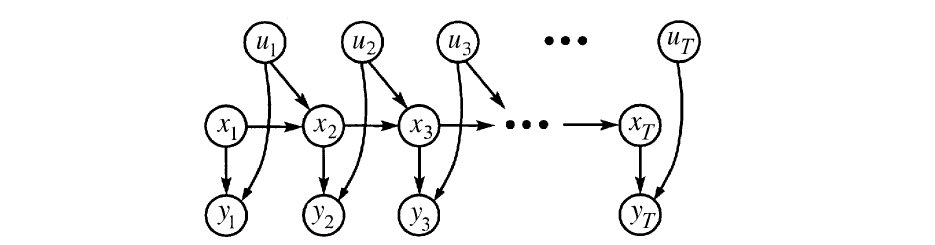
\includegraphics[width=14cm]{screenshot_graphical_model.PNG}
	\captionof{figure}{Graphical model of our system.}
\end{figure}
